\begin{frame}
    \frametitle{Getting Started}

    First, we need to open a command line. The command line (also known as a terminal or console) is
    an invaluable tool for executing text commands on a computer.
    \medskip
    
    \begin{columns}
        \begin{column}{.45\textwidth}
            \begin{block}{Windows}
                From the Start Menu, open the \texttt{Git Bash} application:
                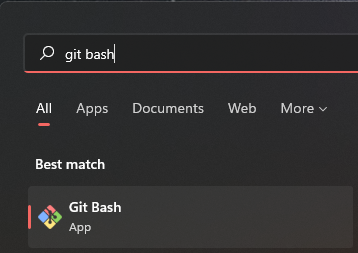
\includegraphics[width=\textwidth]{images/windows_gitbash.png}
            \end{block}
        \end{column}

        \begin{column}{.45\textwidth}
            \begin{block}{MacOS}
                Open the \texttt{Terminal} application from Launchpad:
                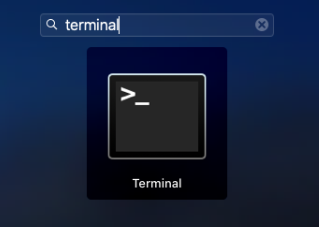
\includegraphics[width=\textwidth]{images/macos_terminal.png}
            \end{block}
        \end{column}
    \end{columns}
\end{frame}